\documentclass[12pt,letterpaper]{article}
\usepackage[utf8]{inputenc}
\usepackage[letterpaper, margin=1in, bottom=2.5in, top=2.2in]{geometry}
\usepackage{fancyhdr}
\setlength{\headheight}{15pt}
\setlength{\footskip}{72pt}

\usepackage{xcolor}
\usepackage{amsmath}
\usepackage{anyfontsize}
\usepackage{graphicx}
\usepackage{tikz}
\usepackage{listings}
\usepackage{sourcesanspro}
\renewcommand{\familydefault}{\sfdefault}
\usepackage{fontawesome5}
\usepackage{titlesec}
\usepackage{setspace}
\usepackage{hyperref}
\usepackage{mdframed}
\usepackage{qrcode}
\usetikzlibrary{calc,shapes,positioning}
\usepackage{eso-pic}

% Command for inline code highlighting
\newcommand{\code}[1]{\texttt{\textcolor{accentColor}{#1}}}

\AtBeginDocument{\color{primaryColor}}

% Colors for Python theme
\definecolor{bgColor}{RGB}{13, 17, 23}  % Dark background
\definecolor{primaryColor}{RGB}{255, 255, 255}  % White text
\definecolor{accentColor}{RGB}{68, 171, 255}  % Python blue for main accent
\definecolor{accentColor2}{RGB}{200, 160, 35}  % Mustard yellow for highlighting concepts
\definecolor{pythonSecondary}{RGB}{180, 180, 180}  % Light gray
\definecolor{secondaryColor}{RGB}{230, 235, 240}  % Almost white gray
\definecolor{terminalBg}{RGB}{22, 22, 22}  % Terminal background
\definecolor{terminalFrame}{RGB}{40, 40, 40}  % Terminal frame
\definecolor{lineNumberColor}{RGB}{100, 100, 100}  % Line number color
\definecolor{dividerColor}{RGB}{120, 130, 150}  % Divider color

% Code colors
\definecolor{codeTextColor}{RGB}{255, 255, 255}  % Basic text
\definecolor{codeKeywordColor}{RGB}{68, 171, 255}  % Keywords in Python blue
\definecolor{codeCommentColor}{RGB}{98, 150, 85}  % Comments 
\definecolor{codeStringColor}{RGB}{200, 160, 35}  % Strings in mustard yellow
\definecolor{codeClassColor}{RGB}{78, 201, 176}  % Classes
\definecolor{codeFunctionColor}{RGB}{200, 160, 35}  % Functions in mustard yellow
\definecolor{codeNumberColor}{RGB}{181, 206, 168}  % Numbers

\pagecolor{bgColor}

\hypersetup{
    colorlinks=true,
    linkcolor=accentColor,
    filecolor=accentColor,
    urlcolor=accentColor,
}

% Define Python language for listings
\lstdefinelanguage{Python}{
  keywords={and, as, assert, break, class, continue, def, del, elif, else, except, finally, for, from, global, if, import, in, is, lambda, nonlocal, not, or, pass, raise, return, try, while, with, yield, async, await},
  sensitive=true,
  comment=[l]{\#},
  morestring=[b]',
  morestring=[b]"
}

% Listings configuration
\lstset{
  language=Python,
  basicstyle=\ttfamily\bfseries\color{codeTextColor},
  backgroundcolor=\color{terminalBg},
  commentstyle=\color{codeCommentColor},
  keywordstyle=\color{codeKeywordColor},
  stringstyle=\color{codeStringColor},
  numberstyle=\color{lineNumberColor},
  breaklines=true,
  breakatwhitespace=true,
  tabsize=4,
  showstringspaces=false,
  frame=none,
  xleftmargin=15pt,
  xrightmargin=0pt,
  aboveskip=5pt,
  belowskip=5pt,
  numbers=left,
  numbersep=8pt,
  extendedchars=true,
  keepspaces=true,
  columns=flexible,
  lineskip=2pt,
  emph={[2]print,len,type,id,dict,list,tuple,set,str,int,float,bool,None,True,False},
  emphstyle={[2]\color{codeFunctionColor}}
}

\newenvironment{macterminal}{%
    \begin{mdframed}[
        linecolor=terminalFrame,
        backgroundcolor=terminalBg,
        roundcorner=5pt,
        skipabove=5pt,
        skipbelow=5pt,
        linewidth=1pt,
        innertopmargin=5pt,
        frametitle={%
            \tikz[baseline=(current bounding box.east), outer sep=0pt]{
                \fill[red!80!black] (0,0) circle (5pt);
                \fill[yellow!80!black] (0.7,0) circle (5pt);
                \fill[green!70!black] (1.4,0) circle (5pt);
            }
        },
        frametitlealignment=\raggedright,
        frametitleaboveskip=8pt,
        frametitlebelowskip=0pt,
    ]
}{%
    \end{mdframed}%
}

\newcommand{\verspace}{\vspace{5pt}}
\newcommand{\languagetag}[1]{
    \begin{tikzpicture}[baseline]
        \node[fill=accentColor, text=primaryColor, rounded corners=5pt, inner sep=7pt] {
            {\normalsize\textbf{#1}}
        };
    \end{tikzpicture}
}

% Title formatting
\titleformat{\section}
  {\LARGE\bfseries\color{primaryColor}}
  {\thesection. }
  {0pt}
  {}
  []

\titleformat{\subsection}
  {\Large\bfseries\color{accentColor}}
  {\thesubsection. }
  {0pt}
  {}
  []

\titleformat{\subsubsection}
  {\large\bfseries\color{accentColor2}}
  {\thesubsubsection. }
  {0pt}
  {}
  []

\titlespacing*{\section}{0pt}{18pt}{8pt}
\titlespacing*{\subsection}{0pt}{12pt}{5pt}
\titlespacing*{\subsubsection}{0pt}{8pt}{3pt}

% Header and footer setup
\pagestyle{fancy}
\fancyhf{}

\fancyhead[L]{
    \begin{tikzpicture}[remember picture, overlay]
        \fill[accentColor, rounded corners=3pt] (0,0) rectangle (2.2cm,0.7cm);
        \node[text=primaryColor, font=\bfseries] at (1.1cm,0.35cm) {PYTHON};
        \fill[primaryColor] (2.35cm,0.1cm) rectangle (2.40cm,0.6cm);
        \node[text=primaryColor, font=\bfseries, anchor=west] at (2.35cm,0.35cm) {NAMESPACES};
    \end{tikzpicture}
}

\renewcommand{\headrulewidth}{0pt}
\renewcommand{\footrulewidth}{0.2pt}
\renewcommand{\footruleskip}{1cm}

\fancyfoot[C]{
    \vspace*{0.1cm}
    \noindent
    \begin{minipage}{\textwidth}
        \begin{flushleft}
            % Profile photo
            \raisebox{0.7cm}{
            \begin{tikzpicture}[baseline]
                \path[fill=bgColor] (0,0) circle (0.6cm);
                \clip (0,0) circle (0.6cm);
                \node at (0,0) {
                    
\includegraphics[width=1.2cm,height=1.2cm]{../../Images/profile-image.jpeg}
                };
            \end{tikzpicture}
            }
            % Profile information
            \begin{minipage}[b]{0.5\textwidth}
                {\large\bfseries\color{primaryColor}Alejandro Sánchez Yalí}
                \par\vspace{1pt}
                {\small\color{secondaryColor}Software Developer | AI \& Blockchain Enthusiast}
                \par\vspace{1pt}
                {\small\color{accentColor2}\faGlobe\hspace{5pt}\color{secondaryColor}www.asanchezyali.com}
            \end{minipage}
        \end{flushleft}
        \vspace{6pt}
    \end{minipage}
}

\fancypagestyle{plain}{
    \fancyhf{}
    \renewcommand{\headrulewidth}{0pt}
    \renewcommand{\footrulewidth}{0pt}
}

\renewcommand{\labelitemi}{\textcolor{accentColor}{$\bullet$}}
\renewcommand{\labelitemii}{\textcolor{accentColor2}{$\circ$}}

\usepackage{relsize}
\AtBeginDocument{\relsize{1}}

% Command for elegant QR
\newcommand{\elegantqr}[2]{
    \qrcode[height=2.5cm]{#1}
    \\[0.1cm]
    {\hspace{0.2cm}\color{primaryColor}\small #2\par}
}


\newcommand{\BackgroundPic}{%
    \put(0,0){%
        \begin{tikzpicture}[remember picture, overlay]
            \node[inner sep=0pt] at (current page.center) {
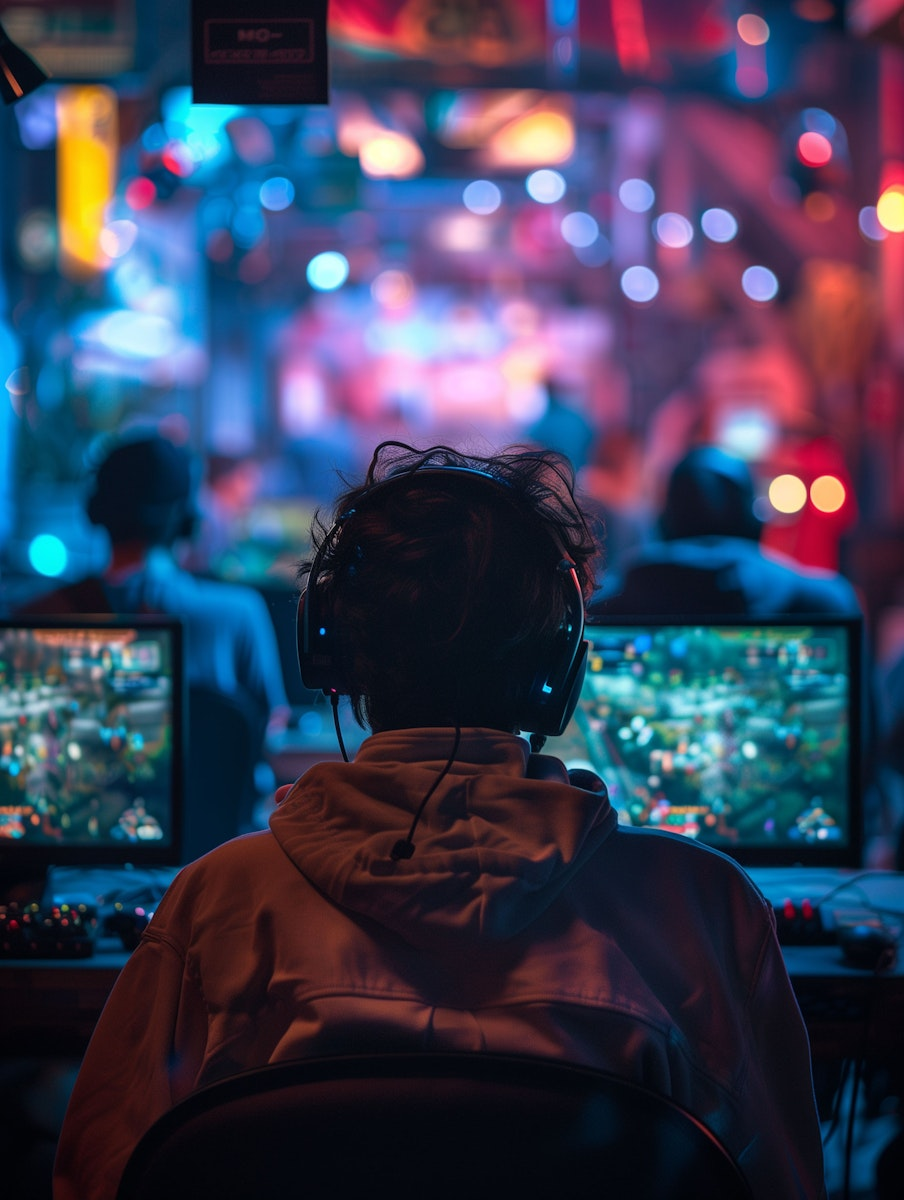
\includegraphics[width=\paperwidth,height=\paperheight,keepaspectratio=false]{../../Images/Arcade Gamer in Action.jpeg}
            };
            \fill[black, opacity=0.7] (current page.south west) rectangle (current page.north east);
        \end{tikzpicture}%
    }%
}

\newcommand{\titlepagecontents}{%
    \AddToShipoutPicture*{\BackgroundPic}
    \vspace*{2cm}
    \begin{flushleft}
    \languagetag{Python}\\[0.4cm]
    {\fontsize{38}{52}\bfseries\color{primaryColor}Understanding \color{accentColor}Python\\\color{accentColor}Namespaces\par}
    \vspace{0.3cm}
    {\fontsize{18}{52}\color{secondaryColor}A Deep Dive into Python's Name Resolution\par}
    \vspace{0.3cm}
    {\color{secondaryColor}\today\par}
    \vspace{1.8cm}
    \elegantqr{https://github.com/asanchezyali/social-media-posts/tree/main/Python/Namespaces}{Source Code}
    \end{flushleft}
}

\newcommand{\finalpagecontents}{%
    \AddToShipoutPicture*{\BackgroundPic}
    \vspace*{3cm}
    \begin{flushleft}
    \languagetag{Feedback}\\[0.4cm]
    {\fontsize{46}{52}\bfseries\color{primaryColor}Found this \color{accentColor}helpful?\par}
    \vspace{0.3cm}
    {\fontsize{18}{52}\color{secondaryColor}Save, comment and share\par}  
    \vspace{0.3cm}
    {\color{secondaryColor}\today\par}
    \end{flushleft}
}

\begin{document}
\setlength{\parindent}{0pt}
\begin{titlepage}
    \titlepagecontents
\end{titlepage}

\section{Understanding Python Namespaces}

In Python, a namespace is a container that holds a mapping of names to objects. Think of it as a dictionary where variable names are the keys and the objects they refer to are the values. Understanding namespaces is crucial because they:

\begin{itemize}
    \item Prevent naming conflicts by organizing names into hierarchical spaces
    \item Define the scope and lifetime of variables
    \item Help manage the visibility and accessibility of variables
\end{itemize}

\section{Types of Namespaces}

Python has several types of namespaces with different lifetimes:

\begin{itemize}
    \item \textbf{Built-in Namespace:} Contains built-in functions and exceptions
    \item \textbf{Global Namespace:} Module-level variables and functions
    \item \textbf{Local Namespace:} Names inside functions
    \item \textbf{Enclosing Namespace:} Names in outer functions (for nested functions)
\end{itemize}

Let's explore each type with practical examples:

\subsection{Basic Namespace Example}

\textbf{How to Run:}
\begin{itemize}
    \item Save the code as \verb|01_basic_namespaces.py|
    \item Run: \verb|python3 01_basic_namespaces.py|
\end{itemize}

\begin{macterminal}
\lstinputlisting[language=Python]{codes/01_basic_namespaces.py}
\end{macterminal}

Key points about this example:
\begin{itemize}
    \item Built-in functions like \texttt{len} live in the built-in namespace
    \item Variables defined at module level (\code{x} and \code{y}) are in the global namespace
    \item Variables defined inside functions (\code{z}) are in the local namespace
    \item The \code{global} keyword allows modifying global variables from inside functions
\end{itemize}

\subsection{Nested Scopes and the nonlocal Keyword}

Let's explore how Python handles nested function scopes and the usage of the \texttt{nonlocal} keyword:

\textbf{How to Run:}
\begin{itemize}
    \item Save the code as \verb|02_nested_scopes.py|
    \item Run: \verb|python3 02_nested_scopes.py|
\end{itemize}

\begin{macterminal}
\lstinputlisting[language=Python]{codes/02_nested_scopes.py}
\end{macterminal}

This example demonstrates:
\begin{itemize}
    \item Local assignments do not affect variables in outer scopes
    \item \code{nonlocal} allows modifying variables in the nearest enclosing scope
    \item \code{global} allows modifying variables in the global scope
    \item Each function has its own local namespace
\end{itemize}

\subsection{Class and Instance Namespaces}

Python also has special namespaces for classes and instances. Let's explore how they work:

\textbf{How to Run:}
\begin{itemize}
    \item Save the code as \verb|03_class_namespaces.py|
    \item Run: \verb|python3 03_class_namespaces.py|
\end{itemize}

\begin{macterminal}
    \lstinputlisting[language=Python]{codes/03_class_namespaces.py}
\end{macterminal}

Key points about class and instance namespaces:
\begin{itemize}
    \item Class variables are shared among all instances
    \item Instance variables are unique to each instance
    \item Be cautious with mutable class variables
    \item Python looks up attributes first in the instance namespace, then in the class namespace
\end{itemize}

\section{Advanced Namespace Concepts: Closures and Annotations}

Python's namespace system becomes even more powerful when working with closures and type annotations. These advanced features demonstrate the flexibility and sophistication of Python's scoping rules.

\subsection{Function Closures and Free Variables}

A closure occurs when a nested function references variables from its enclosing scope. The inner function "closes over" the variables it needs, preserving them even after the outer function returns.

\textbf{How to Run:}
\begin{itemize}
    \item Save the code as \verb|04_closures_annotations.py|
    \item Run: \verb|python3 04_closures_annotations.py|
\end{itemize}

\begin{macterminal}
    \lstinputlisting[language=Python]{codes/04_closures_annotations.py}
\end{macterminal}

This example demonstrates several advanced concepts:

\begin{itemize}
    \item Each function call creates a new instance of the local variables
    \item Closures can "remember" values from the enclosing scope  
    \item The \code{nonlocal} keyword is needed to modify enclosed variables
    \item Type annotations in closures follow special scoping rules
\end{itemize}

\subsection{Key Insights About Closures}

When working with closures in Python:

\begin{itemize}
    \item Each function call creates a new instance of the local variables
    \item Closures can "remember" values from the enclosing scope
    \item The \code{nonlocal} keyword is needed to modify enclosed variables
    \item Type annotations in closures follow special scoping rules
\end{itemize}

\subsection{Best Practices with Closures}

When using closures in your code:

\begin{itemize}
    \item Use closures to create functions with private state
    \item Be careful with mutable free variables
    \item Consider using default arguments for early binding when needed
    \item Document the closure's behavior and any captured variables
\end{itemize}

\section{Name Resolution Rules: LEGB}

Python follows the LEGB rule when looking up names:

\begin{itemize}
    \item \textbf{Local}: Names declared inside the current function
    \item \textbf{Enclosing}: Names in enclosing functions
    \item \textbf{Global}: Names declared at module level
    \item \textbf{Built-in}: Names in the built-in module
\end{itemize}

Python searches these namespaces in this order until it finds the name or raises a \code{NameError}.

\section{Best Practices}

When working with namespaces in Python:

\begin{itemize}
    \item Use \code{global} sparingly - it can make code harder to understand
    \item Prefer passing values as arguments and returning results
    \item Be careful with mutable class variables
    \item Use clear and descriptive names to avoid confusion
    \item Document when you need to use \code{global} or \code{nonlocal}
\end{itemize}

\section{References}

\begin{itemize}
    \item Python Documentation. (2025). \textit{Python Scopes and Namespaces}.
    \href{https://docs.python.org/3/tutorial/classes.html#python-scopes-and-namespaces}{Link}
    
    \item Python Documentation. (2025). \textit{The global statement}. 
    \href{https://docs.python.org/3/reference/simple_stmts.html#the-global-statement}{Link}
    
    \item Python Documentation. (2025). \textit{The nonlocal statement}. 
    \href{https://docs.python.org/3/reference/simple_stmts.html#the-nonlocal-statement}{Link}
    
    \item Lutz, M. (2023). \textit{Learning Python, 6th Edition}. O'Reilly Media.
    
    \item This article was edited and written in collaboration with AI. If you find any inconsistencies or have suggestions for improvement, please don't hesitate to open an issue in our \href{https://github.com/asanchezyali/social-media-posts}{GitHub} repository or reach out directly.
\end{itemize}

\section{Explore More Python Concepts}
\vspace{10pt}
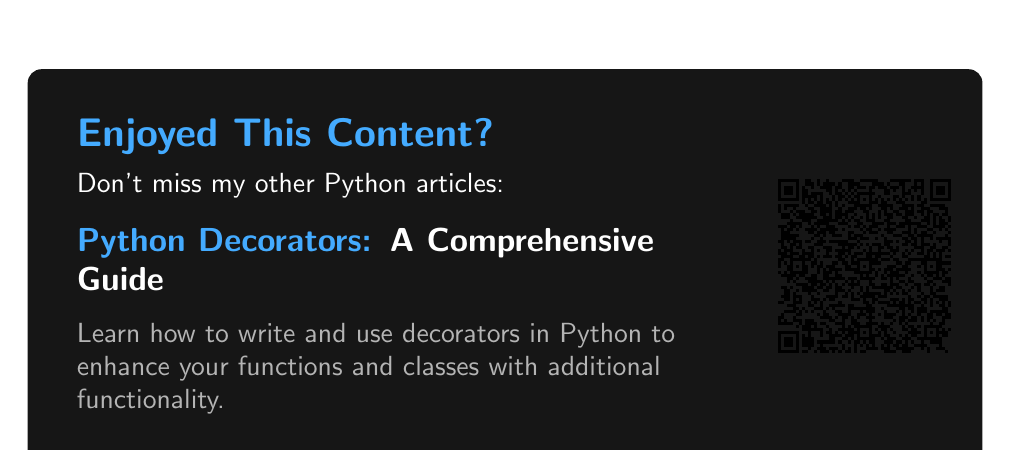
\begin{tikzpicture}
    \fill[color=terminalBg, rounded corners=5pt] (0,0) rectangle (\textwidth,-5);
    
    \pgfmathsetmacro{\availableWidth}{\textwidth-4cm}
    
    \begin{scope}
        \node[text=accentColor, font=\Large\bfseries, anchor=north west] at (0.5cm,-0.5cm) {Enjoyed This Content?};
        
        \node[text=primaryColor, font=\normalsize, anchor=north west] at (0.5cm,-1.2cm) {Don't miss my other Python articles:};
        
        \node[text=secondaryColor, font=\large\bfseries, anchor=north west, text width=\availableWidth] at (0.5cm,-1.9cm)
            {\color{accentColor}Python Decorators: \color{primaryColor}A Comprehensive Guide};
        
        \node[text=pythonSecondary, font=\normalsize, text width=\availableWidth, anchor=north west] at (0.5cm,-3.1cm) {
            Learn how to write and use decorators in Python to enhance your functions and classes with additional functionality.
        };
    \end{scope}
    
    \node[anchor=center] at ({\textwidth-1.5cm}, {-2.5cm}) {
        \qrcode[height=2.2cm]{https://www.linkedin.com/posts/asanchezyali_python-decorators-activity-7304916650070364160-xWFL?utm_source=share&utm_medium=member_desktop&rcm=ACoAACfC_XIB4R901-Rs4Cep7e9KjyGl5ZhS47o}
    };
    
\end{tikzpicture}
\vspace{5pt}

\clearpage
\thispagestyle{empty}
\finalpagecontents

\end{document}